\documentclass{IEEEoj}
\usepackage{cite}
\usepackage{amsmath,amssymb,amsfonts}
\usepackage{graphicx,color}
\usepackage{textcomp}
\usepackage{url}
\usepackage[ruled,vlined]{algorithm2e}
\def\BibTeX{{\rm B\kern-.05em{\sc i\kern-.025em b}\kern-.08em
    T\kern-.1667em\lower.7ex\hbox{E}\kern-.125emX}}
\def\OJlogo{\vspace{-10pt}
\includegraphics[height=20pt]{OJAP.png}}
\begin{document}
\receiveddate{XX Month, XXXX}
\reviseddate{XX Month, XXXX}
\accepteddate{XX Month, XXXX}
\publisheddate{XX Month, XXXX}
\currentdate{XX Month, XXXX}
\doiinfo{OJAP.2020.1234567}

\title{Ray-tracing Based RIS Size, Position and Target Point Optimization for Indoor Coverage Enhancement}

\author{EMRE KILCIOGLU, AND CLAUDE OESTGES}
\corresp{ICTEAM/ELEN, Universit\'e catholique de Louvain, Louvain-la-Neuve, Belgium\\\\
	CORRESPONDING AUTHOR: E. KILCIOGLU (e-mail: emre.kilcioglu@uclouvain.be)}
\authornote{This study was conducted as part of the project Win2Wal2023/1 - N°2310026 - RAFINE, funded by Région Wallonne.}
\markboth{Ray-tracing Based RIS Size, Position and Target Point Optimization for Indoor Coverage Enhancement}{Kilcioglu \textit{et al.}}

\begin{abstract}
....
\end{abstract}

\begin{IEEEkeywords}
......
\end{IEEEkeywords}

%\IEEEspecialpapernotice{(Invited Paper)}

\maketitle

\section{INTRODUCTION}
\IEEEPARstart{T}{his} .....

\section{RIS INTEGRATION INTO THE RAY-TRACING TOOL}
This section outlines the integration of an RIS into the ray-tracing simulation tool. We choose to work with NVIDIA's open-source Sionna ray-tracing tool \cite{sionna} due to its user-friendly structure and the ability to change internal parameters of the tool according to our use.

In an indoor environment, transmitter-only coverage maps reveal blind spots which are the areas with inadequate signal quality caused by obstacles such as walls or large furniture that block line-of-sight (LoS) paths between the transmitter and these regions. To address this, an RIS can be strategically positioned to create virtual LoS paths, reflecting signals from the transmitter to these blind spots. By configuring the RIS to direct reflected signals into these areas, the average signal power in blind spots and the overall coverage ratio can be improved through the combined contributions of the transmitter and RIS. In this paper, the considered performance metric is the average power of these blind spots, and the aim is to maximize this metric by optimizing the position, size, and target point selection of the RIS.

To incorporate the RIS into the ray-tracing tool, the surface is discretized into a grid of $N \times M$ tiles, each with dimensions $d_y$ and $d_z$, as shown in Fig. \ref{RIS_Modeling}. Each tile, denoted as $T_{n,m}$ for the $n^{\text{th}}$ row and $m^{\text{th}}$ column, is characterized by a complex reflection coefficient that controls the amplitude and phase of incoming electromagnetic waves to reflect the signal to the desired target points. The discretization approach approximates a continuous surface when $d_y$ and $d_z$ are sufficiently small, which provides precise control over the reflected wavefronts. Without loss of generality, in this paper, the RIS is assumed to be placed in the y-z plane of the 3D simulation scenario.

The RIS's reflection behavior is determined by the collective contribution of its tiles, which are configured to reflect signals toward $K \geq 1$ target points. For simplicity, Fig. \ref{RIS_Modeling} illustrates a single target point, although we consider multiple target points in this paper to address multiple blind spots. The complex reflection coefficient for a single tile, $\Gamma_{n,m}$, is expressed as
\begin{equation} \label{ref_coef_exp}
	\Gamma_{n,m} = \sum \limits_{k=1}^K \sqrt{c_k} A_{n,m}^k e^{j \varphi_{n,m}^k}
\end{equation}
where $A_{n,m}^k$ and $\varphi_{n,m}^k$ represent the amplitude and phase assigned for the $k^{\text{th}}$ target point, respectively. These assignments collectively form the 2D amplitude profile $\mathbf{A}^k$ and the phase profile $\mathbf{\Phi}^k$ for the RIS to reflect the signal into the $k^{\text{th}}$ target point. The power intensity coefficient $c_k$, which determines the power allocated to each target point, satisfies the following:
\begin{equation}
	\sum_{k=1}^K c_k = 1
\end{equation}
The overall reflection coefficient $\mathbf{\Gamma}$ of the RIS is computed as the weighted sum of the individual amplitude and phase profiles for all target points, with weights given by the power intensity coefficients $c_k$.

The considered RIS modeling enables the simulation of various RIS configurations in different environments. For instance, in complex indoor scenarios with significant obstructions, the RIS can mitigate blind spots by steering reflected signals around obstacles into otherwise unreachable areas. Through careful design of amplitude and phase profiles, the RIS enhances received signal power in these areas and addresses shadowing effects.

\begin{figure}
	\centering 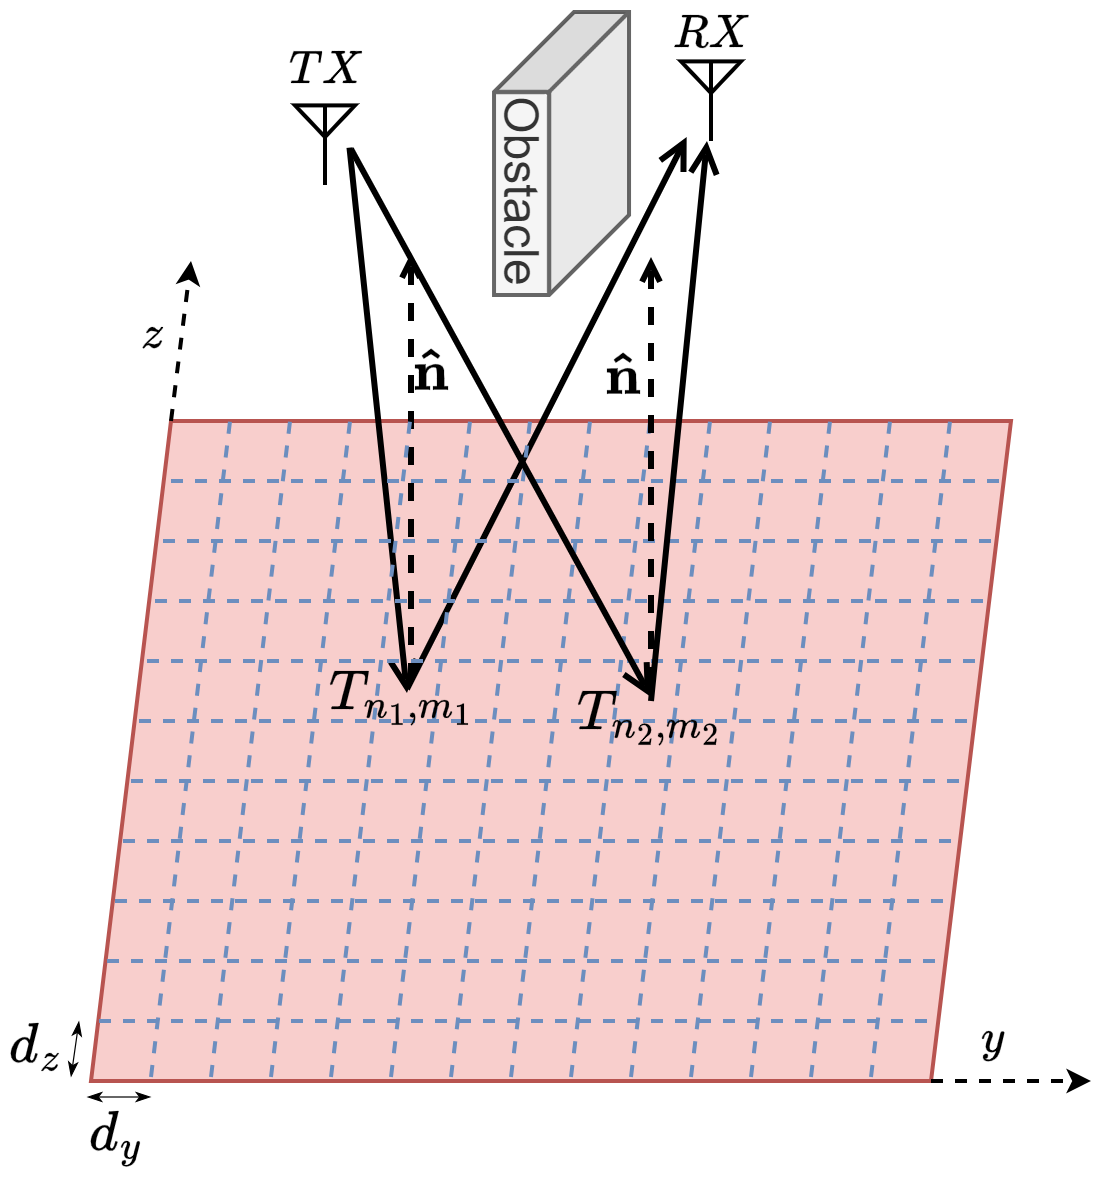
\includegraphics[width=.8\linewidth]{RIS_Modeling.png}
	\caption{Illustration of RIS modeling: The RIS surface is discretized into tiles, each with tunable reflection characteristics, to direct signals toward the target points.}
	\label{RIS_Modeling}
\end{figure}

\section{RIS PHASE PROFILE CONFIGURATION METHODS}
In RIS modeling, the primary focus is on the phase change introduced to the incoming signal, as the amplitude is typically assumed to remain constant, generally between $0.8$ and $1$. Therefore, the design and optimization of RIS are centered on assigning appropriate phase profiles to control the direction and behavior of reflected waves.

In this section, we consider two primary methods for configuring the phase profiles $\mathbf{\Phi}^k$ of the RIS to achieve anomalous reflections for each target point $k$: the gradient-based phase profile \cite{phase_grad_paper} and the distance-based phase profile \cite{Tang}. These methods offer distinct advantages, making them suitable for different environmental scenarios and system requirements.

\begin{enumerate}
	\item \textbf{Gradient-based Phase Profile}: This method considers the incidence and desired reflection wave directions, and it aims to achieve the desired reflection direction by introducing a phase gradient across the RIS. The phase gradient is computed to align the reflected signal with the desired reflection direction, thereby optimizing the coverage at the target points.
	
	\item \textbf{Distance-based Phase Profile}: In contrast to the gradient-based method, the distance-based method focuses on the total distance traveled by the incident and reflected signals. By adjusting the phase shifts to match the distances from the transmitter to each tile and from each tile to a specific target point, the method ensures that the reflected signals constructively interfere at this target point location.
\end{enumerate}

The phase profile for these methods is computed for each target point $k$, and the individual phase profiles are combined through the summation in (\ref{ref_coef_exp}) to derive the overall reflection coefficient profile $\mathbf{\Gamma}$.

\subsection{GRADIENT-BASED PHASE PROFILE}
The gradient-based method, as illustrated in Fig. \ref{RIS_Phase_Gradient}, treats the RIS as an ideal phase gradient reflector. The phase gradient is calculated based on the incident wave direction and the desired reflection direction for each target point. In this method, the RIS introduces a phase gradient that modifies the direction of the reflected waves, aiming to direct the reflected signal toward a desired target point.

Let us consider an incident wave with wave vector $\mathbf{\hat{k}}_i$ arriving at the center of the RIS at an incidence angle $\theta_i$ with respect to the RIS normal vector $\mathbf{\hat{n}}$. The desired reflection direction for the target point $k$ is represented by the reflection wave vector $\mathbf{\hat{k}}_r$ with a reflection angle $\theta_r$. The incident phase gradient due to the inclined wavefront is given by
\begin{equation} \label{grad_phi_i}
	\nabla \varphi_i = - k_0 \sin\theta_i \, \mathbf{\hat{k}}_i^p = - k_0 \, \textbf{P} \mathbf{\hat{k}}_i
\end{equation}
where $k_0 = 2 \pi / \lambda$ is the wavenumber and $\lambda$ is the wavelength. Here, $\mathbf{\hat{k}}_i^p$ represents the unit projection of the incident wave vector $\mathbf{\hat{k}}_i$ onto the plane of the RIS, and $\textbf{P}$ is the projection operator, where $\textbf{P} \mathbf{\hat{k}}_i = \sin\theta_i \, \mathbf{\hat{k}}_i^p$.

The RIS applies an additional phase gradient $\nabla \varphi_{RIS}$, which adjusts the reflection direction to achieve the desired angle $\theta_r$. Then, the reflection phase gradient $\nabla \varphi_r$ becomes
\begin{equation} \label{grad_phi}
	\nabla \varphi_r = \nabla \varphi_i + \nabla \varphi_{RIS}
\end{equation}
Similar to (\ref{grad_phi_i}), the reflection phase gradient $\nabla \varphi_r$ is expressed as
\begin{equation} \label{grad_phi_r}
	\nabla \varphi_r = - k_0 \ \sin\theta_r \ \mathbf{\hat{k}}_r^p = - k_0 \ \textbf{P} \mathbf{\hat{k}}_r
\end{equation}
where $\mathbf{\hat{k}}_r^p$ is the unit projection vector of the reflection wave vector \( \mathbf{\hat{k}}_r \) onto the RIS. By substituting (\ref{grad_phi_i}) and (\ref{grad_phi_r}) into (\ref{grad_phi}), we find the desired phase gradient onto the RIS to reflect the incoming wave with direction $\mathbf{\hat{k}}_i$ to the reflection wave with direction $\mathbf{\hat{k}}_r$
\begin{equation} \label{grad_exp}
	\nabla \varphi_{RIS} = k_0 \ \textbf{P} (\mathbf{\hat{k}}_i - \mathbf{\hat{k}}_r) = k_0 \ (\sin\theta_i \ \mathbf{\hat{k}}_i^p - \sin\theta_r \ \mathbf{\hat{k}}_r^p)
\end{equation}
For simpler cases, such as when the RIS, transmitter, and target positions are assumed to be at the same height, the phase gradient onto the RIS becomes one-dimensional along the y-axis, which can be shown as follows:
\begin{equation} \label{grad_exp_simpler}
	\nabla \varphi_{RIS} = k_0 \, (\sin\theta_i - \sin\theta_r) \, \hat{y}
\end{equation}
This simplification results in a one-dimensional phase gradient and a more straightforward implementation of the RIS design.

The phase profile $\mathbf{\Phi}^k$ for each target point $k$ is then generated by setting the first RIS tile phase to zero and applying a linear variation of the phase across the surface, following the gradient calculated in (\ref{grad_exp}) or (\ref{grad_exp_simpler}). 

\begin{figure}
	\centering 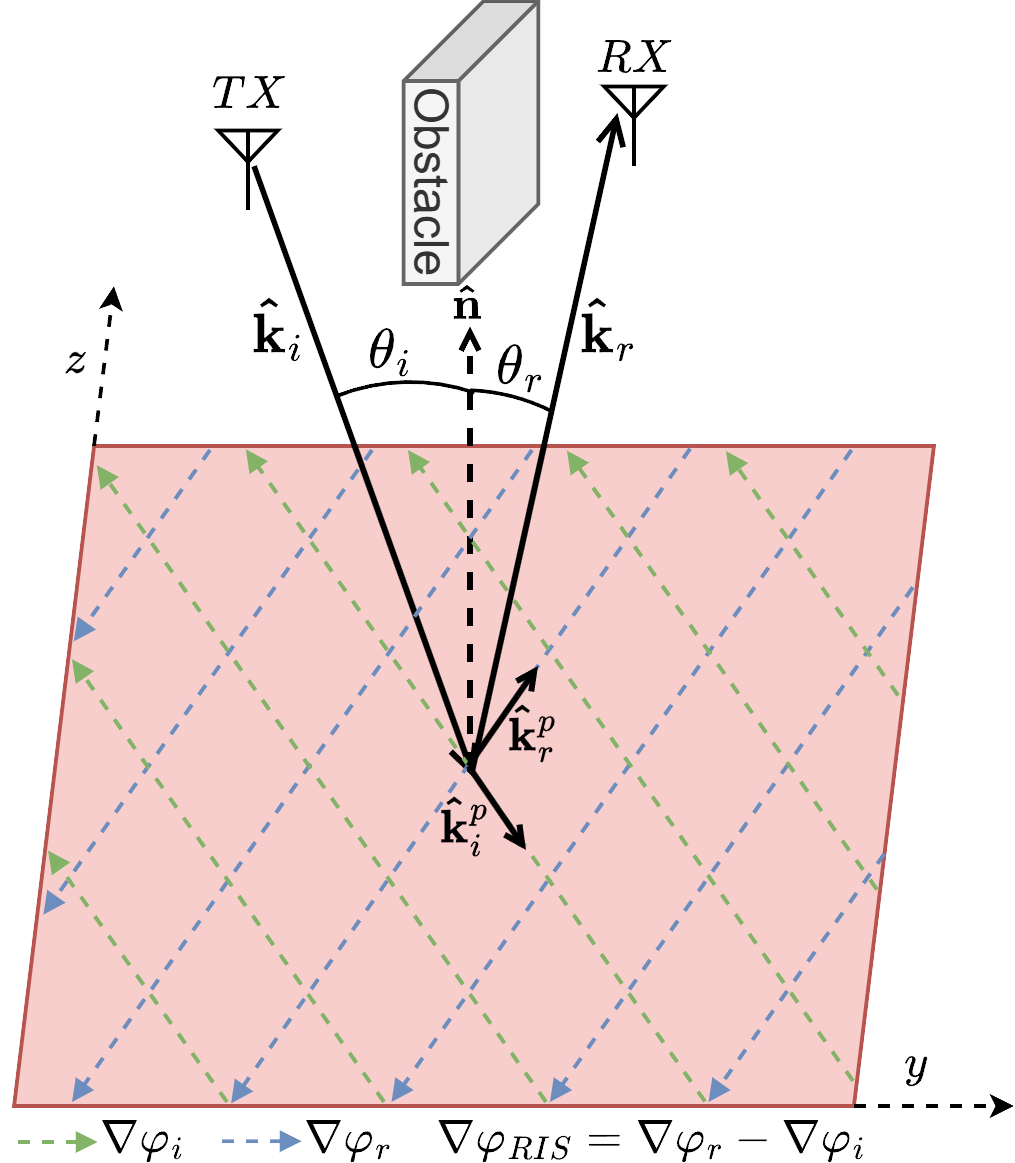
\includegraphics[width=\linewidth]{RIS_Phase_Gradient.png}
	\caption{The gradient-based method for configuring the RIS phase profile to reflect signals toward the target point}
	\label{RIS_Phase_Gradient}
\end{figure}

\subsection{DISTANCE-BASED PHASE PROFILE}
The distance-based method models the RIS as a focusing lens that ensures the reflected signals combine constructively at the target point. By calculating the phase shift required at each tile, this method ensures that the signals from all tiles travel the same total distance, ensuring constructive interference at the target point.

The position of each tile $T_{n,m}$ relative to the RIS center is given by $(0, (m-\frac{1}{2})d_y, (n-\frac{1}{2})d_z)$, where $m \in \left[ 1 - \frac{M}{2}, \frac{M}{2} \right]$ and $n \in \left[ 1 - \frac{N}{2}, \frac{N}{2} \right]$ represent the row and column indices of the tile, assuming that the center of the coordinate system is taken as the center of the RIS without loss of generality.

The electric field arriving at each tile $T_{n,m}$ is expressed as
\begin{equation}
	E_{n,m}^{\text{in}} = \sqrt{\frac{2 Z_0 P_{n,m}^{\text{TX-RIS}}}{d_y d_z}} e^{-j \frac{2 \pi r_{n,m}^{tx}}{\lambda}}
\end{equation}
where $Z_0$ is the characteristic impedance of free space, $r_{n,m}^{tx}$ is the distance between the transmitter and $T_{n,m}$, and $P_{n,m}^{\text{TX-RIS}}$ is the received power of the incident wave at each tile. After reflection, the total electric field at the desired target point is
\begin{equation}
	E^{rx} = \sum_{n=1-\frac{N}{2}}^{\frac{N}{2}} \sum_{m=1-\frac{M}{2}}^{\frac{M}{2}} E_{n,m}^{rx}
\end{equation}
where each reflected field, contributed by $T_{n,m}$ is:
\begin{equation} \label{E_n_m_r}
	E_{n,m}^{rx} = \sqrt{\frac{2 Z_0 P^{rx}_{n,m}}{A_{rx}}} e^{-j \left(\frac{2 \pi}{\lambda} (r_{n,m}^{tx} + r_{n,m}^{rx}) - \varphi_{n,m}^k\right)}
\end{equation}
where $r_{n,m}^{rx}$ is the distance from $T_{n,m}$ to the receiver, $A_{rx}$ is the receiving antenna aperture, and $P_{n,m}^{rx}$ is the power of the reflected signal of $T_{n,m}$ at the desired target point and can be expressed as
\begin{equation}
	P_{n,m}^{rx} = P_{n,m}^{\text{RIS-RX}} (A_{n,m}^k)^2 P_{n,m}^{\text{TX-RIS}}
\end{equation}
where $P_{n,m}^{\text{RIS-RX}}$ is the multiplicative factor to the received power of the path from $T_{n,m}$ to the desired target point. The combined received power of all tiles at target point $k$ is then given by
\begin{equation} \label{combined_rx_power}
	\begin{aligned}
		P^{rx} &= \frac{\left|E^{rx}\right|^2}{2 Z_0} A_{rx} \\
		&= \left| \sum_{n=1-\frac{N}{2}}^{\frac{N}{2}} \sum_{m=1-\frac{M}{2}}^{\frac{M}{2}} A_{n,m}^k \sqrt{P_{n,m}^{\text{TX-RIS}} P_{n,m}^{\text{RIS-RX}}} \right. \\
		&\quad \left. \times e^{-j \left(\frac{2 \pi}{\lambda} (r_{n,m}^{tx} + r_{n,m}^{rx}) - \varphi_{n,m}^k\right)} \right|^2
	\end{aligned}
\end{equation}
In the distance-based phase profile method, the aim is to maximize the combined received power $P^{rx}$ in (\ref{combined_rx_power}), which is maximized when the imaginary part of each term in the summation is tuned in. Then, the following phase assignment for each tile holds:
\begin{equation}
	\varphi_{n,m}^k = \frac{2 \pi}{\lambda} (r_{n,m}^{tx} + r_{n,m}^{rx})
\end{equation}
where the phase profile $\mathbf{\Phi}^k$ is created by assigning this expression to each tile to achieve constructive interference at the desired target point.

\section{JOINT RIS SIZE, POSITION AND TARGET POINT OPTIMIZATION ALGORITHM} \label{algo_section}
In a typical indoor scenario, the transmitter's position is assumed to be fixed in this paper. Then, we can easily simulate the transmitter-only coverage map in the ray-tracing tool and reveal the scenario's blind spots with insufficient signal power that require coverage enhancement. The objective of this study is to utilize RIS deployment to improve the signal power in these blind spots, ensuring acceptable signal quality throughout all the areas in the scene.

In our previous work \cite{emre_claude_eucap_paper}, we addressed this issue by introducing a method to identify blind spots based on the transmitter-only coverage map. By defining a minimum power threshold for acceptable signal quality, regions with power levels below this threshold were classified as low-power cells which require coverage enhancement. The coordinates of these low-power cells were then grouped into a fixed number of clusters using the K-means clsutering algorithm, and the centroids of these clusters were selected as the target points for the RIS. However, the position of the RIS in \cite{emre_claude_eucap_paper} was assumed to be fixed, which limited the flexibility of the solution.

To overcome this limitation, we propose a novel algorithm in this study that jointly optimizes the RIS size, position, and number of target points. The algorithm first identifies low-power cells based on the transmitter-only coverage map. For each possible number of target points, it searches for feasible RIS positions within the scene that maintain a line-of-sight (LoS) connection with both the transmitter and all target points. Each feasible configuration of RIS position and number of target points is evaluated for each searched RIS size. The best configuration defined by the RIS position and number of target points is selected for each RIS size. Subsequently, the RIS size is varied iteratively, and the performance improvement is assessed. When the performance improvement falls below the defined threshold, the corresponding RIS size is selected as the sub-optimal size. This approach not only seeks to improve coverage but also balances performance gains with hardware cost by determining a sub-optimal RIS size. Increasing the RIS size enhances coverage, but after a certain point, the performance improvement becomes marginal compared to the added cost. Hence, the proposed algorithm identifies the trade-off point between performance and cost by defining a performance improvement threshold. This threshold manages the decision to continue increasing the RIS size. Without loss of generality, this study varies the RIS size by adjusting its width while keeping its height fixed, allowing for a clear analysis of one-dimensional size variations. However, the approach can be extended to two-dimensional size adjustments, where both height and width are increased proportionally. Detailed steps of the proposed algorithm are presented in Algorithm \ref{algo1}-\ref{algo2}.

\begin{algorithm}
	\caption{Ray-tracing Based RIS Size, Position and Target Points Optimization (Part 1)}
	\label{algo1}
	\SetAlgoLined
	\KwIn{
		\begin{itemize}
			\item \textbf{The scene geometry:} A 3D representation of the area where coverage is to be enhanced, including obstacles, walls, etc.
			\item \textbf{Transmitter (TX) position:} Coordinates of the transmitter in the scene.
			\item \textbf{Minimum power threshold} $P_{\text{th}}$: The threshold for acceptable signal power, below which cells are considered low-power.
			\item \textbf{Range of possible target points} $\mathcal{N}$: The set of possible cluster counts to be used in K-means algorithm, e.g., $\mathcal{N} = \{1, 2, \dots, 5\}$.
			\item \textbf{Set of possible RIS widths} $\mathcal{W}$: The set of candidate RIS widths, e.g., $\mathcal{W} = \{0.2, 0.4, \dots, 3.0\}$ m.
			\item \textbf{Minimum performance improvement threshold} $\Delta \mathcal{M}_{\text{min}}$: The minimum performance improvement required to justify increasing the RIS width.
		\end{itemize}
	}
	\KwOut{
		\begin{itemize}
			\item \textbf{Sub-optimal number of target points} $N^{\text{opt}}$.
			\item \textbf{Sub-optimal RIS width} $W_{\text{RIS}}^{\text{opt}}$.
			\item \textbf{Sub-optimal RIS position} $\mathbf{r}_{\text{RIS}}^{\text{opt}}$.
		\end{itemize}
	}
	Compute the transmitter-only coverage map $\mathbf{P}_{\text{TX}}(x, y)$.\\
	Set a minimum power threshold $P_{\text{th}}$ for acceptable signal quality.\\
	Identify low-power cells in $\mathbf{P}_{\text{TX}}(x, y)$ where the power level is below the minimum power threshold $P_{\text{th}}$, denoted as $\mathcal{C}_{\text{low}}$:
	\begin{equation}
		\mathcal{C}_{\text{low}} = \{(x, y) \ | \ \mathbf{P}_{\text{TX}}(x, y) < P_{\text{th}}\}
	\end{equation}
\end{algorithm}

\begin{algorithm}
	\caption{Ray-tracing Based RIS Size, Position and Target Points Optimization (Part 2)}
	\label{algo2}
	\SetAlgoLined
	\ForEach{number of target points $N \in \mathcal{N}$}{
		Apply K-means algorithm to $\mathcal{C}_{\text{low}}$ to group the low-power cells into $N$ clusters and obtain $N$ centroids:
		\begin{equation}
			\text{K-means}(N, \mathcal{C}_{\text{low}}) \rightarrow \text{Centroids} \{ \mathbf{c}_1, \mathbf{c}_2, \dots, \mathbf{c}_N \}
		\end{equation}
		where each centroid $\mathbf{c}_i$ represents a target point where coverage enhancement is needed.\\
		Identify the set of feasible RIS positions $\mathcal{R}_N$ that provide line-of-sight (LoS) to both the transmitter and all $N$ target points:
		\begin{equation}
			\mathcal{R}_N = \{ \mathbf{r}_{\text{RIS}} \mid \text{LoS}(\mathbf{r}_{\text{RIS}}, \mathbf{TX}) \land \text{LoS}(\mathbf{r}_{\text{RIS}}, \mathbf{c}_i) \ \forall \mathbf{c}_i \}
		\end{equation}
		\ForEach{RIS width $W_{\text{RIS}} \in \mathcal{W}$}{
			Compute the combined coverage $\textbf{P}_{\text{comb}}(x,y)$ at each low-power cell, considering both TX and RIS contributions, for each RIS position $\mathbf{r}_{\text{RIS}} \in \mathcal{R}_N$.\\
			Calculate the performance metric $\mathcal{M}(\mathbf{r}_{\text{RIS}}, N, W_{\text{RIS}})$ for all parameter combinations as the average power of low-power cells after placing the RIS at $\mathbf{r}_{\text{RIS}}$:
			\begin{equation}
				\mathcal{M}(\mathbf{r}_{\text{RIS}}, N, W_{\text{RIS}}) = \frac{1}{|\mathcal{C}_{\text{low}}|} \sum_{(x, y) \in \mathcal{C}_{\text{low}}} \mathbf{P}_{\text{comb}}(x, y)
			\end{equation}
		}
	}
	
	Identify the RIS configuration $(\mathbf{r}_{\text{RIS}}^{W_{\text{RIS}}}, N^{W_{\text{RIS}}}, W_{\text{RIS}})$ that maximizes the performance metric $\mathcal{M}$ for each $W_{\text{RIS}}$:
	\begin{equation}
		(\mathbf{r}_{\text{RIS}}^{W_{\text{RIS}}}, N^{W_{\text{RIS}}}) = \arg\max_{\mathbf{r}_{\text{RIS}} \in \mathcal{R}_N, N \in \mathcal{N}} \mathcal{M}(\mathbf{r}_{\text{RIS}}, N, W_{\text{RIS}})
	\end{equation}\\
	Select the smallest RIS width $W_{\text{RIS}}^{\text{opt}}$ for which increasing the RIS width further does not yield a performance improvement exceeding $\Delta \mathcal{M}_{\text{min}}$. Assign corresponding parameters $\mathbf{r}_{\text{RIS}}^{\text{opt}} = \mathbf{r}_{\text{RIS}}^{W_{\text{RIS}}^{\text{opt}}}$ and $N^{\text{opt}} = N^{W_{\text{RIS}}^{\text{opt}}}$.
\end{algorithm}

\section{SIMULATION RESULTS}

\subsection{SIMULATION SCENARIO}
In this paper, we consider a U-shaped indoor office scenario consisting of three main hallways: the 'upper' and 'lower' hallways, which form the two arms of the U, and the 'intersecting' hallway that connects them at the bottom. Additionally, there is an internal room located at the intersection of these hallways. The layout of the scenario is illustrated in Fig. \ref{Scenario}, where the transmitter position is marked with a blue circle, and an example RIS placement is represented by a purple rectangle on the intersecting hallway wall.

For the simulation environment, the materials used for the walls, floors, and ceilings are selected from a predefined list in Sionna RT, based on their typical usage in indoor environments and their electromagnetic properties. Sionna RT incorporates material models defined in the ITU-R P.2040-2 recommendation \cite{ITU}. Specifically, the selected materials are:  
\begin{itemize}
	\item \textbf{Walls:} Plasterboard (\textit{itu\_plasterboard}) is chosen due to its common application in building interiors.
	\item \textbf{Floors:} Chipboard (\textit{itu\_chipboard}) is selected for its suitability and practicality as an indoor flooring material.
	\item \textbf{Ceilings:} Ceiling board (\textit{itu\_ceiling\_board}) is used for its specific design for ceilings.
\end{itemize}

In this scenario, the transmitter is assumed to be placed at the intersection of the hallways on the upper side, as indicated by the blue circle in Fig. \ref{Scenario}. This placement may result in potential blind spots with weak signal quality at the far edge of the lower hallway and certain areas within the internal room. To mitigate these blind spots, an RIS can be strategically positioned on the wall of the intersecting hallway, depending on the selected minimum power threshold value.

\begin{figure}
	\centering 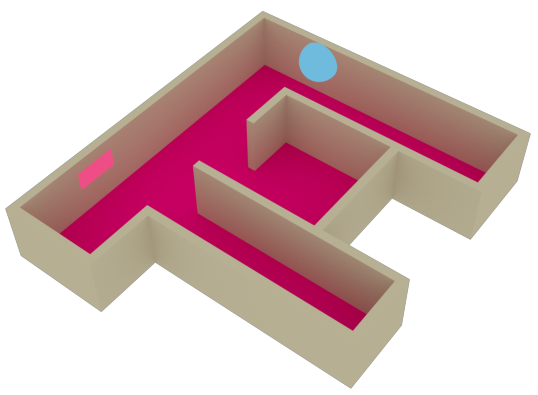
\includegraphics[width=.8\linewidth]{Sim_Results/Scenario_Illustration.png}
	\caption{Scenario Illustration}
	\label{Scenario}
\end{figure}

\subsection{GRAPHICAL USER INTERFACE (GUI) FOR SIMULATION RESULTS EXTRACTION}
A Python-based graphical user interface (GUI) has been developed to facilitate the extraction and visualization of simulation results for the proposed algorithm. The main interface of this GUI is shown in Fig. \ref{GUI}. This interface allows users to load predefined scenarios, define the operating frequency of the scene, set the position of the transmitter, specify the minimum power threshold, and configure numerous other parameters.

After the necessary parameters are entered, the GUI provides several functionalities, including:  
\begin{itemize}
	\item Generating coverage map plots.
	\item Identifying the RIS target points using the K-means clustering algorithm, based on the distribution of low-power cells in the transmitter-only coverage map.
	\item Displaying feasible RIS positions depending on the location of the target points.
\end{itemize}

Furthermore, the GUI allows users to define the boundaries for optimization parameters related to the proposed algorithm in Section \ref{algo_section}. These parameters include the number of target points, RIS width, and RIS position. The GUI computes performance metrics for all possible combinations of these parameters, enabling users to end up with sub-optimal optimization configurations. Additionally, the GUI can visualize the effect of RIS width on performance metrics, as well as generate cumulative distribution functions (CDFs) for different phase profile approaches and RIS sizes.

The GUI is shared as an open-source project on GitHub and can be accessed at the following link:  
\url{https://github.com/ekilcioglu/RIS-Optimization-GUI}

\begin{figure}
	\centering 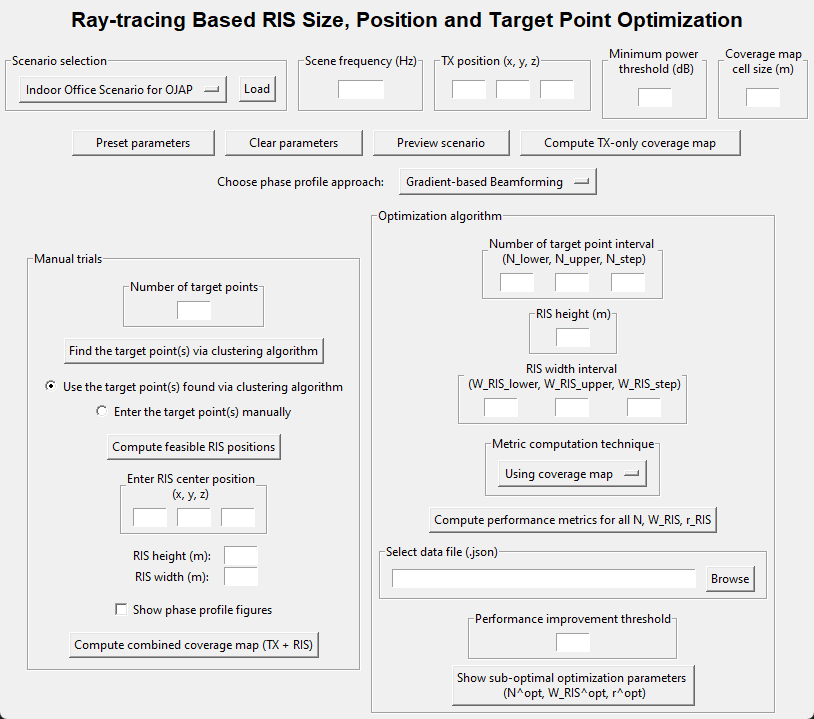
\includegraphics[width=\linewidth]{Sim_Results/GUI.png}
	\caption{Illustration of the GUI interface}
	\label{GUI}
\end{figure}

\subsection{SIMULATION PARAMETERS}
The simulation parameters are carefully chosen to evaluate the performance of the proposed algorithm under realistic conditions. The amplitude profile of the reflection coefficients for each target point is set to unity to isolate and analyze the pure effect of the phase profiles. The power intensity coefficients, $c_k$, which determine how power is distributed among the target points, are set to equal values, ensuring identical importance is assigned to each blind spot in the scenario.

The system operates at a communication frequency of $5.8$ GHz, corresponding to a wavelength of $\lambda = c/f = 5.17$ cm, where $c$ is the speed of light. The RIS grid sizes, $d_y$ and $d_z$, are defined as $\lambda / 2 = 2.585$ cm.

Two distinct minimum power threshold values $P_{\text{th}}$ are considered in the simulations:  
\begin{itemize}
	\item $-100$ dB: This threshold results in a higher number of low-power cells in the scene, providing a broader area for the RIS to enhance.
	\item $-110$ dB: This lower threshold value allows the RIS to focus on cells with comparably weaker power levels.
\end{itemize}

The results corresponding to these threshold values are simulated separately to assess the impact of power thresholds on the optimization and coverage enhancement provided by the RIS.

\subsection{TRANSMITTER-ONLY COVERAGE MAP}
The transmitter-only coverage map, which represents the power distribution from the transmitter without the assistance of an RIS, is depicted in Fig. \ref{TX_coverage_map}. The transmitter position is marked with a red '+' sign. As observed in the figure, signal power decreases significantly in certain areas of the scenario, resulting in potential blind spots with weak signal coverage.

Specifically, these blind spots are primarily located at the far edge of the lower hallway and in several regions within the internal room. The presence of these blind spots highlights the limitations of transmitter-only coverage in complex indoor environments with non-line-of-sight (NLOS) regions and significant signal attenuation caused by obstacles and walls. Such weak coverage can negatively impact the reliability and quality of communication in these areas.

To address these limitations, the strategic placement of an RIS becomes essential. By redirecting and enhancing the signal, the RIS can extend the coverage to include these blind spots, thereby improving the overall system performance. The selection of an optimal RIS placement depends on factors such as the spatial distribution of the low-power cells in the blind spots and the minimum power threshold values used in the simulations.

Fig. \ref{TX_coverage_map} serves as the baseline coverage map, against which the improvements brought by the RIS placement and optimization will be evaluated in subsequent sections.

\begin{figure}
	\centering 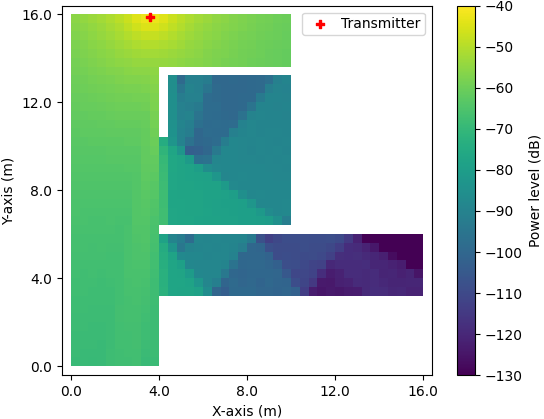
\includegraphics[width=.9\linewidth]{Sim_Results/TX_coverage_map.png}
	\caption{Transmitter-only coverage map}
	\label{TX_coverage_map}
\end{figure}

\subsection{RESULTS FOR MINIMUM POWER THRESHOLD OF $-100$ dB}

\subsubsection{BINARY POOR COVERAGE MAPS FOR DIFFERENT NUMBER OF TARGETS}
For the simulations, we begin by assigning a minimum power threshold of $-100$ dB. As explained earlier, cells in the coverage map that fall below this threshold are categorized as low-power cells, which require a power boost for reliable communication. The distribution of these low-power cells is depicted in Fig. \ref{binary_maps} for different numbers of target points $N$. These plots, referred to as binary poor coverage maps, visually represent the areas where the signal strength is below the threshold (red areas) and areas where the signal strength is acceptable (blue areas).

The positions of the low-power cells are clustered using the K-means algorithm, and the centroids of these clusters are marked as green 'x' symbols in Fig. \ref{binary_maps}. These centroids represent the target points where the RIS will steer its beams to improve signal coverage. Feasible RIS positions are then determined based on line-of-sight (LoS) visibility to both the target points and the transmitter. These positions are indicated by green star symbols on the same figure.

For each configuration shown in Fig. \ref{binary_maps}, the average power of the low-power cells is calculated as $-112.58$ dB, significantly below the set minimum power threshold of $-100$ dB.

In addition to the average power of the low-power cells, we also analyze a new metric known as the coverage ratio. The coverage ratio represents the percentage of the scene that is covered by either the transmitter or the RIS. The coverage ratio in the transmitter-only coverage map for the consideration of the minimum power threshold of $-100$ dB is $81.54\%$, as seen in Fig. \ref{binary_maps}. This coverage ratio metric is crucial, as focusing only on the average power of low-power cells might lead to misleading results. For example, a higher average power could indicate an improvement in performance, but if many areas remain uncovered, the coverage ratio could still be limited. A situation like this might arise if the RIS concentrates on boosting the power of certain low-power cells, thus increasing their signal strength significantly, while leaving other low-power cells uncovered. Monitoring the coverage ratio reveals such scenarios and helps ensure that the optimization does not overlook areas that still lack coverage.

Although this issue can occur, it is generally rare because the RIS initially boosts the power level of any low-power cell it illuminates. However, after a certain point, focusing further on the same cell does not result in exponential power increases, as the RIS effect becomes saturated.

\begin{figure}
	\centering
	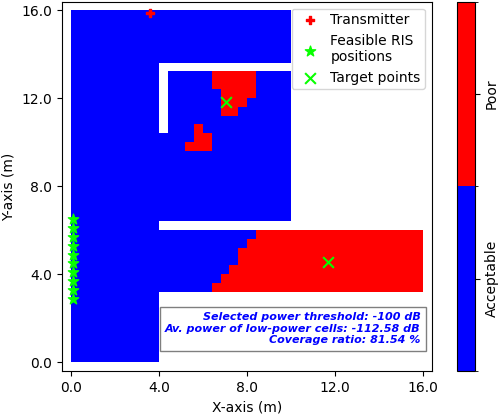
\includegraphics[width=0.49\linewidth]{Sim_Results/Binary_Cov_Map_N_2_-100dB.png}
	\hfill
	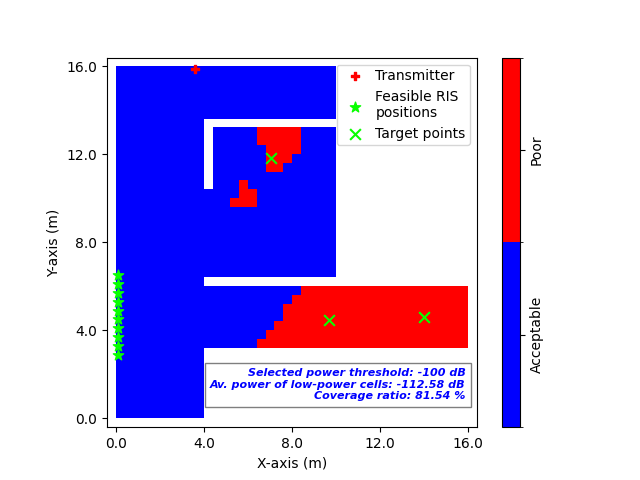
\includegraphics[width=0.49\linewidth]{Sim_Results/Binary_Cov_Map_N_3_-100dB.png}
	
	a) $N = 2$ \ \ \ \ \ \ \ \ \ \ \ \ \ \ \ \ \ \ \ \ \ \ \ b) $N = 3$ \\[5pt]
	
	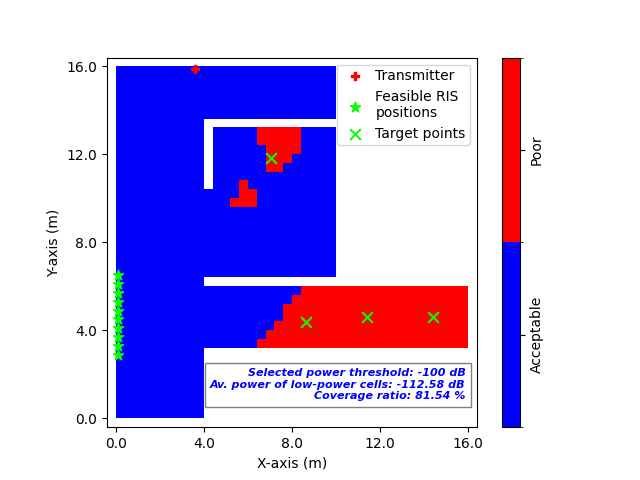
\includegraphics[width=0.49\linewidth]{Sim_Results/Binary_Cov_Map_N_4_-100dB.png}
	\hfill
	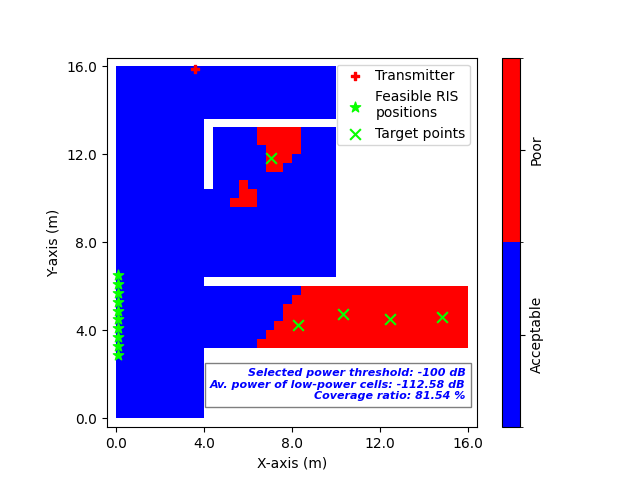
\includegraphics[width=0.49\linewidth]{Sim_Results/Binary_Cov_Map_N_5_-100dB.png}
	
	c) $N = 4$ \ \ \ \ \ \ \ \ \ \ \ \ \ \ \ \ \ \ \ \ \ \ \ d) $N = 5$
	\caption{Binary poor coverage maps for different number of target configurations for the minimum power threshold of $-100$ dB}
	\label{binary_maps}
\end{figure}

\subsubsection{RIS OPTIMIZATION ALGORITHM RESULTS}
After generating the transmitter-only coverage map, identifying the low-power cells, determining the target points, and feasible RIS positions, the optimization algorithm proposed in Section \ref{algo_section} is applied to calculate the performance metric $\mathcal{M}$. This metric is evaluated for all parameter combinations, including the number of target points, feasible RIS positions, and RIS width. For each RIS width, the configuration that maximizes $\mathcal{M}$ is identified as the sub-optimal configuration for that specific width.

The results of the performance metric $\mathcal{M}$ for varying RIS widths are shown in Fig. \ref{perf_metric_RIS_width_multiple_curves_-100dB}, considering different RIS heights and phase profile approaches. It can be observed that the curves tend to saturate beyond a certain RIS width. Initially, increasing the RIS width significantly enhances the coverage by boosting the power level of low-power cells illuminated by the RIS. However, once most of these cells reach an acceptable power level, additional increases in RIS width do not contribute significantly to further improvements. This highlights the importance of considering the cost-effectiveness of increasing RIS width.

Another notable observation is that the gradient-based approach consistently outperforms the distance-based approach for the considered minimum power threshold of $-100$ dB. This is because the gradient-based approach not only boosts the power at the target points but also increases the power at other locations along the beam paths, covering a broader area. In contrast, the distance-based approach aims to create constructive interference specifically at the target points, which results in a more localized effect. While this approach leads to a significant power boost at the selected points, it does not effectively extend coverage to surrounding low-power cells, leaving some areas insufficiently illuminated. Despite this limitation, the distance-based approach still yields a noticeable improvement in performance. This difference between these phase profile approaches is particularly pronounced in scenarios where the low-power regions are large, making the gradient-based approach more effective in such cases.

The impact of RIS height is also more noticeable in the distance-based approach compared to the gradient-based approach. Specifically, when the RIS height is increased from $0.5$ m to $1$ m, the improvement in performance is more significant for the distance-based approach. In contrast, for the gradient-based approach, a smaller RIS height provides nearly equivalent performance, suggesting that a lower RIS height can be selected in such cases to balance performance with practical deployment constraints.

\begin{figure}
	\centering
	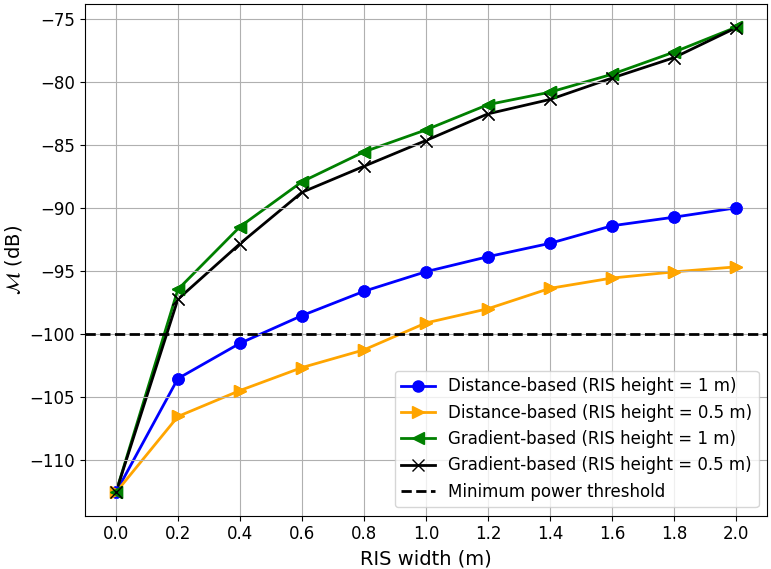
\includegraphics[width=\linewidth]{Sim_Results/perf_metric_RIS_width_multiple_curves_-100dB.png}
	\caption{Performance metric $\mathcal{M}$ as a function of RIS width for different RIS heights and phase profile approaches, with a minimum power threshold of $-100$ dB}
	\label{perf_metric_RIS_width_multiple_curves_-100dB}
\end{figure}

Next, in Fig. \ref{perf_metric_RIS_width_-100dB_gradient_height_1m}, the gradient-based approach for an RIS height of $1$ m is analyzed in detail. The figure highlights the configurations that maximize the performance metric $\mathcal{M}$ for each RIS width. The annotations in the figure indicate the optimal RIS positions (denoted as "RIS pos") and the number of target points for different widths as well as the corresponding coverage ratio. 

To determine the sub-optimal RIS width, a performance improvement threshold $\Delta \mathcal{M}_{\text{min}}$ is introduced. This threshold represents the minimum performance gain required to justify increasing the RIS width to the next level. For example, higher thresholds lead to smaller RIS widths with slightly reduced performance, as increasing the RIS width further does not provide sufficient improvement to justify the additional cost. As seen in Fig. \ref{perf_metric_RIS_width_-100dB_gradient_height_1m}, even a minimal RIS width of $0.2$ m significantly boosts $\mathcal{M}$ compared to the transmitter-only case (No RIS). Furthermore, the coverage ratio improves significantly, reaching nearly $100\%$ at larger RIS widths, demonstrating the effectiveness of the optimization algorithm.

\begin{figure}
	\centering
	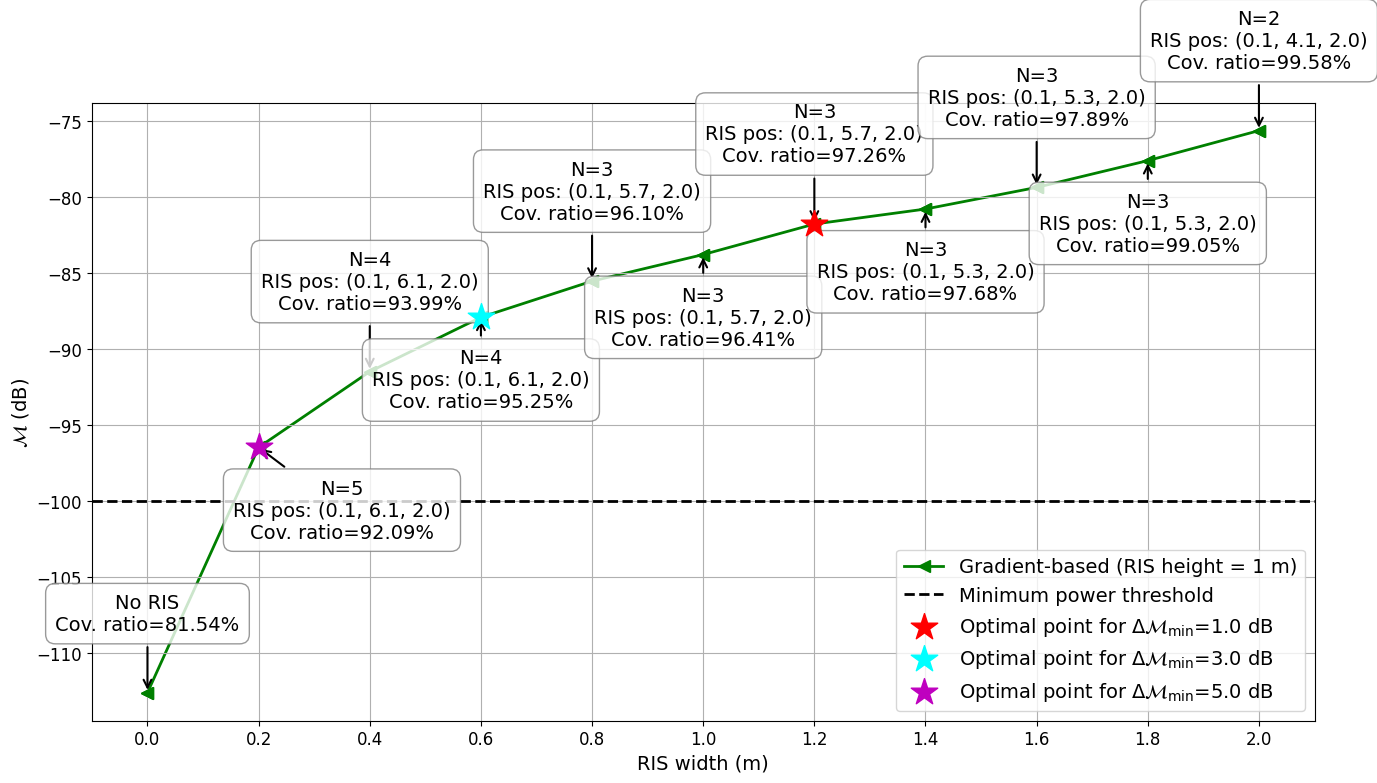
\includegraphics[width=\linewidth]{Sim_Results/perf_metric_RIS_width_-100dB_gradient_height_1m.png}
	\caption{Performance metric $\mathcal{M}$ vs. RIS width for the gradient-based approach, showing selected sub-optimal configurations for different performance improvement thresholds $\Delta \mathcal{M}_{\text{min}}$ with an RIS height of $1$ m and a minimum power threshold of $-100$ dB.}
	\label{perf_metric_RIS_width_-100dB_gradient_height_1m}
\end{figure}

In Fig. \ref{perf_metric_RIS_width_-100dB_distance_height_1m}, the distance-based approach is analyzed for an RIS height of $1$ m. Similar trends are observed, with slightly lower performance metric values and coverage ratios compared to the gradient-based approach. This difference reflects the distance-based approach’s narrower focus on the target points, which leaves some low-power cells uncovered.

\begin{figure}
	\centering
	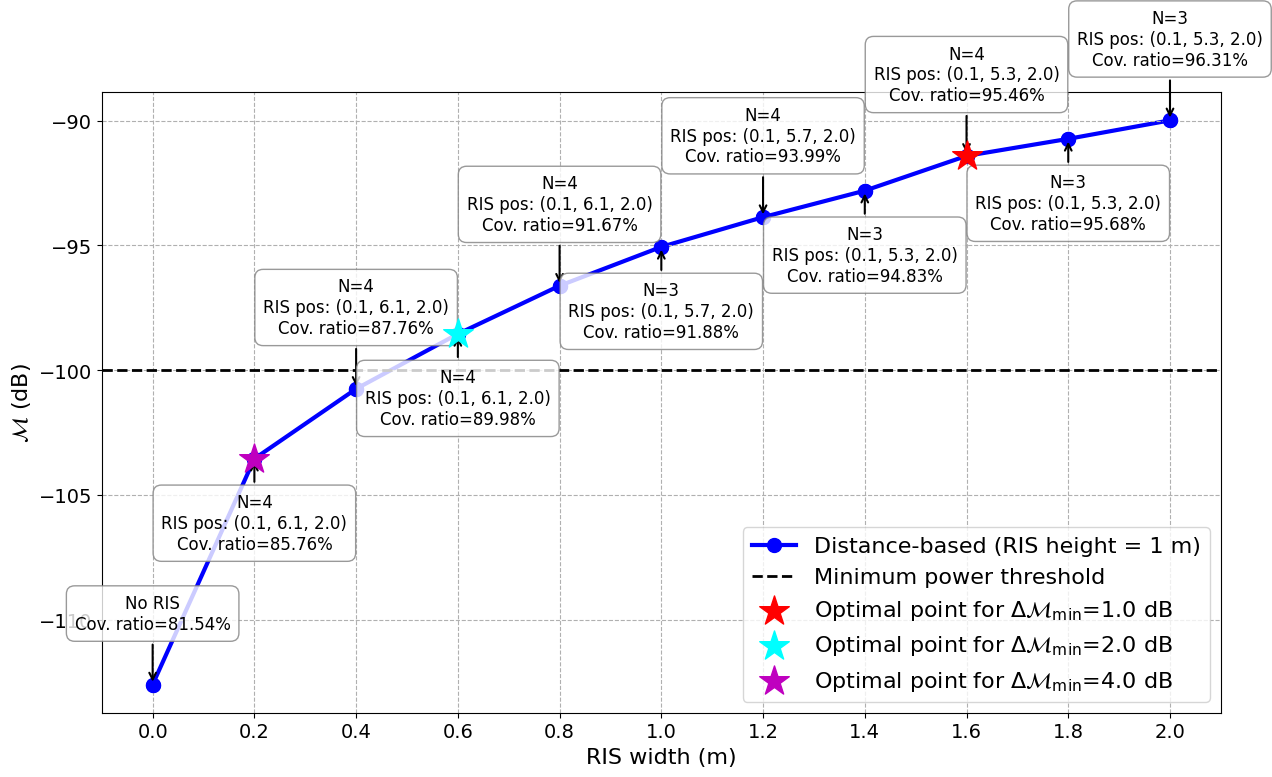
\includegraphics[width=\linewidth]{Sim_Results/perf_metric_RIS_width_-100dB_distance_height_1m.png}
	\caption{Performance metric $\mathcal{M}$ vs. RIS width for the distance-based approach, showing selected sub-optimal configurations for different performance improvement thresholds $\Delta \mathcal{M}_{\text{min}}$ with an RIS height of $1$ m and a minimum power threshold of $-100$ dB.}
	\label{perf_metric_RIS_width_-100dB_distance_height_1m}
\end{figure}

\begin{figure}
	\centering 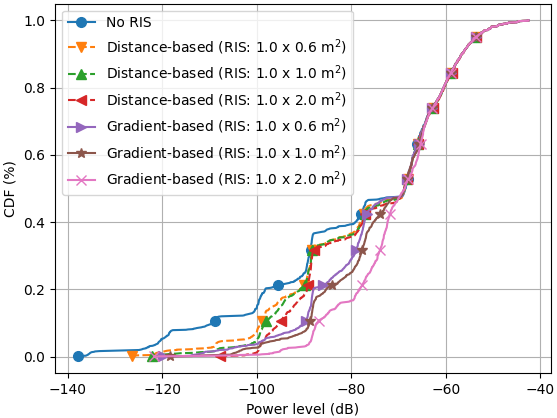
\includegraphics[width=\linewidth]{Sim_Results/CDF_-100dB.png}
	\caption{Cumulative distribution functions (CDFs) for different phase profile approaches and RIS sizes}
	\label{CDF_-100dB}
\end{figure}

\begin{figure}
	\centering
	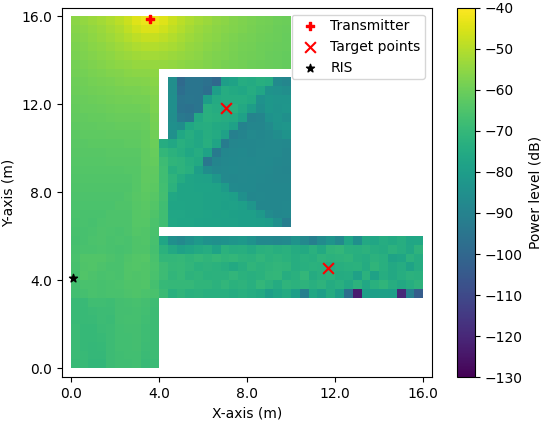
\includegraphics[width=0.7\linewidth]{Sim_Results/Comb_cov_1x2_Gradient.png}
	
	a) Combined coverage map \\[5pt]
	
	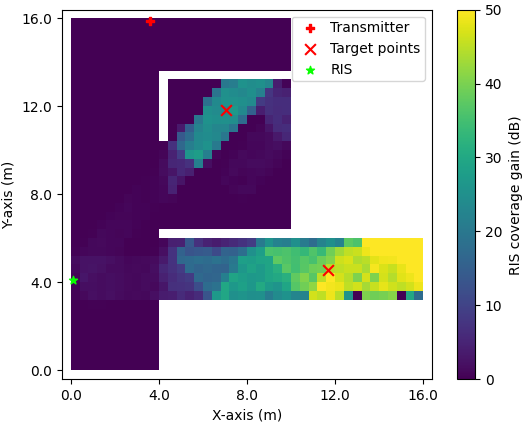
\includegraphics[width=0.49\linewidth]{Sim_Results/RIS_cov_gain_1x2_Gradient.png}
	\hfill
	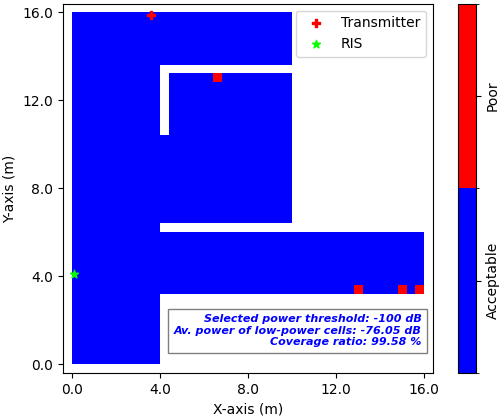
\includegraphics[width=0.48\linewidth]{Sim_Results/New_Binary_Cov_Map_1x2_Gradient.png}
	
	b) RIS coverage gain \ \ \ \ \ \ \ \ \ \ \ c) New binary poor \\ \ \ \ \ \ \ \ \ \ \ \ \ \ \ \ \ \ \ \ \ \ \ \ \ \ \ \ \ \ \ \ \ \ \ \ \ \ \ \ coverage map
	\caption{Combined coverage map of the transmitter and the RIS with the RIS size of $1 \times 2$ m$^2$ by using the gradient-based approach}
	\label{comb_cov_gradient}
\end{figure}

\begin{figure}
	\centering
	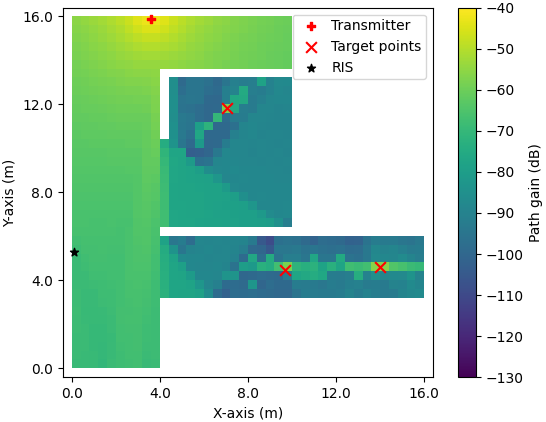
\includegraphics[width=0.7\linewidth]{Sim_Results/Comb_cov_1x2_Distance.png}
	
	a) Combined coverage map \\[5pt]
	
	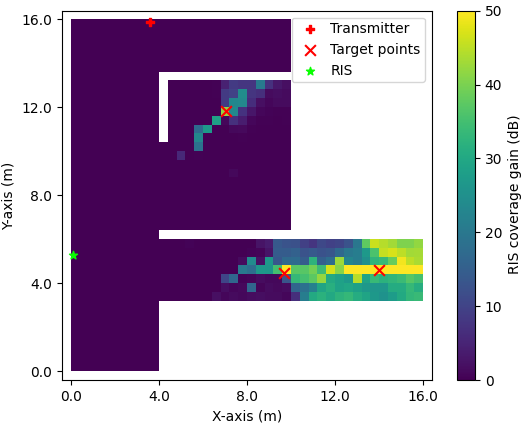
\includegraphics[width=0.49\linewidth]{Sim_Results/RIS_cov_gain_1x2_Distance.png}
	\hfill
	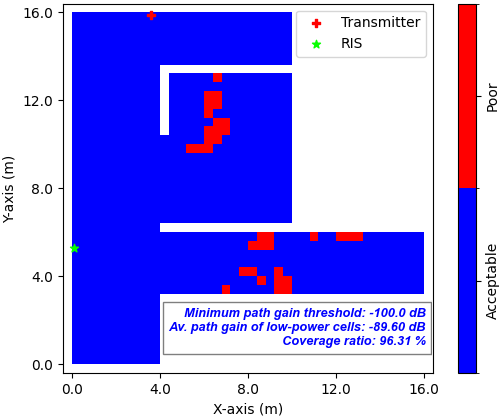
\includegraphics[width=0.48\linewidth]{Sim_Results/New_Binary_Cov_Map_1x2_Distance.png}
	
	b) RIS coverage gain \ \ \ \ \ \ \ \ \ \ \ c) New binary poor \\ \ \ \ \ \ \ \ \ \ \ \ \ \ \ \ \ \ \ \ \ \ \ \ \ \ \ \ \ \ \ \ \ \ \ \ \ \ \ \ coverage map
	\caption{Combined coverage map of the transmitter and the RIS with the RIS size of $1 \times 2$ m$^2$ by using the distance-based approach}
	\label{comb_cov_distance}
\end{figure}

\begin{figure}
	\centering
	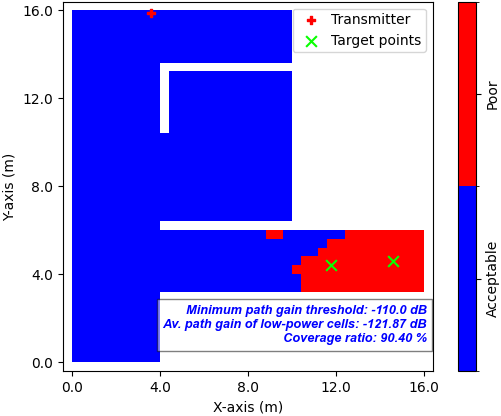
\includegraphics[width=0.49\linewidth]{Sim_Results/Binary_Cov_Map_N_2_-110dB.png}
	\hfill
	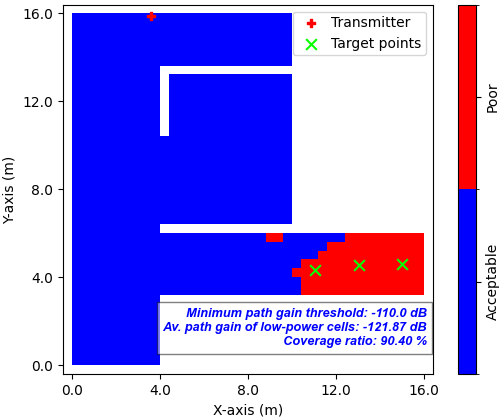
\includegraphics[width=0.49\linewidth]{Sim_Results/Binary_Cov_Map_N_3_-110dB.png}
	
	a) $N = 2$ \ \ \ \ \ \ \ \ \ \ \ \ \ \ \ \ \ \ \ \ \ \ \ b) $N = 3$ \\[5pt]
	
	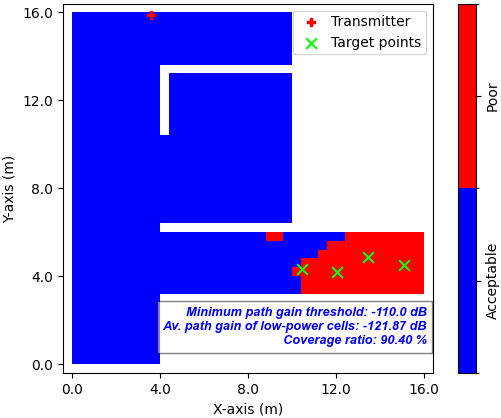
\includegraphics[width=0.49\linewidth]{Sim_Results/Binary_Cov_Map_N_4_-110dB.png}
	\hfill
	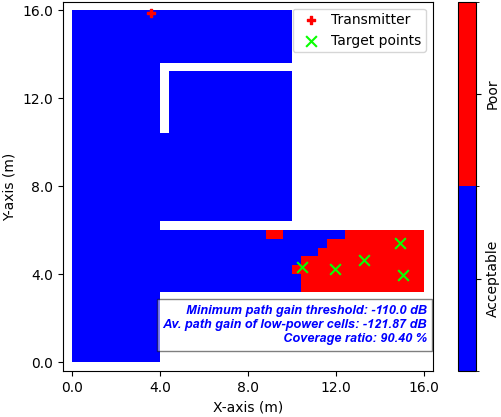
\includegraphics[width=0.49\linewidth]{Sim_Results/Binary_Cov_Map_N_5_-110dB.png}
	
	c) $N = 4$ \ \ \ \ \ \ \ \ \ \ \ \ \ \ \ \ \ \ \ \ \ \ \ d) $N = 5$
	\caption{Binary poor coverage maps for different number of target configurations for $-110$ dB minimum power threshold}
	\label{binary_maps_-110dB}
\end{figure}

\begin{figure}
	\centering 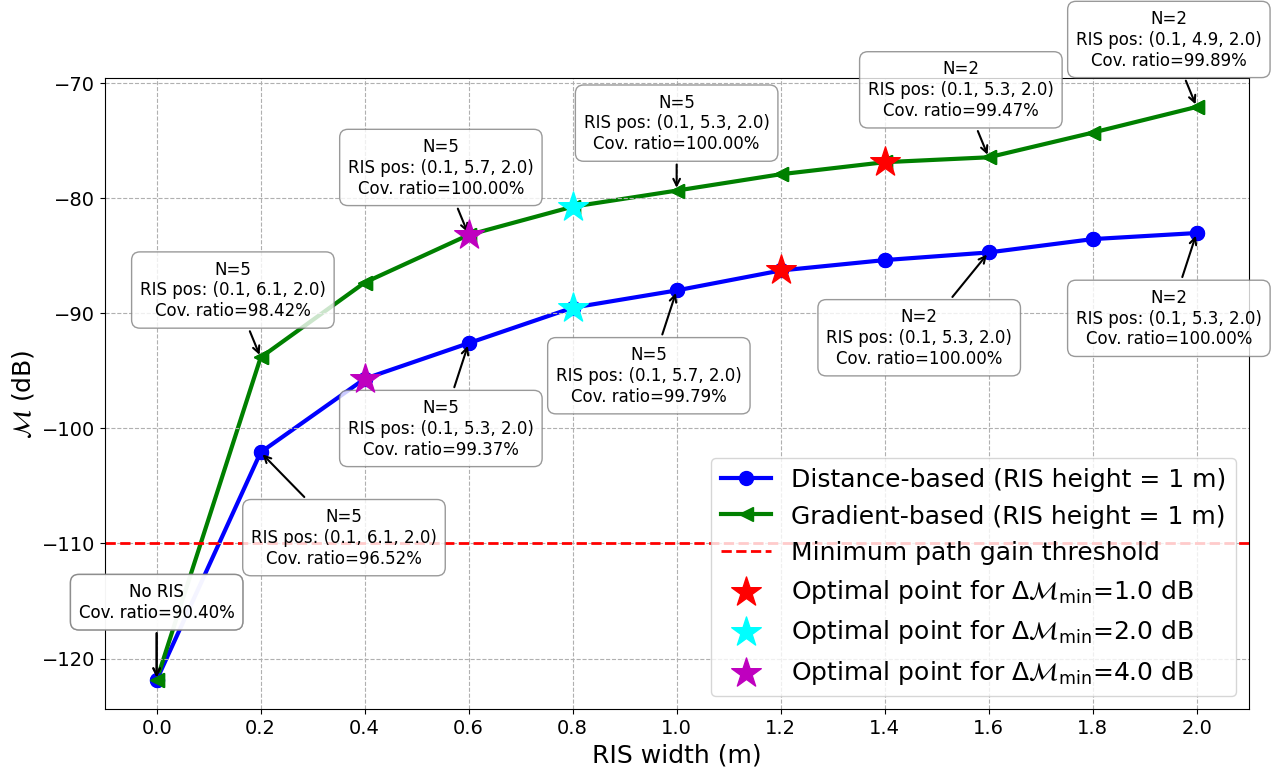
\includegraphics[width=\linewidth]{Sim_Results/perf_metric_RIS_width_-110dB_multiple_curves_height_1m.png}
	\caption{Performance metric $\mathcal{M}$ vs. RIS width and the selected optimal points for different minimum performance improvement thresholds $\Delta \mathcal{M}_{\text{min}}$ for the RIS height of $1$ m for $-110$ dB minimum power threshold}
	\label{perf_metric_RIS_width_-110dB_multiple_curves_height_1m}
\end{figure}

\begin{figure}
	\centering 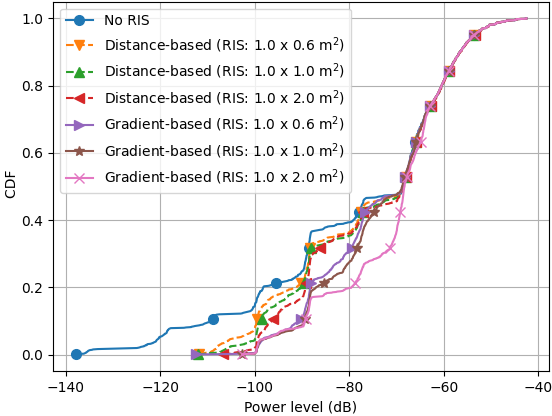
\includegraphics[width=\linewidth]{Sim_Results/CDF_-110dB.png}
	\caption{Cumulative distribution functions (CDFs) for different phase profile approaches and RIS sizes for $-110$ dB minimum power threshold}
	\label{CDF_-110dB}
\end{figure}

\begin{figure}
	\centering
	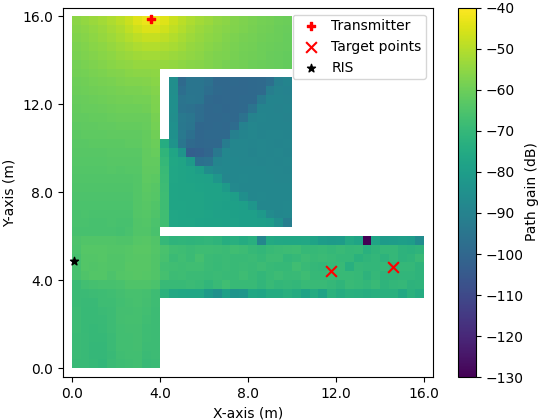
\includegraphics[width=0.7\linewidth]{Sim_Results/Comb_cov_1x2_Gradient_-110dB.png}
	
	a) Combined coverage map \\[5pt]
	
	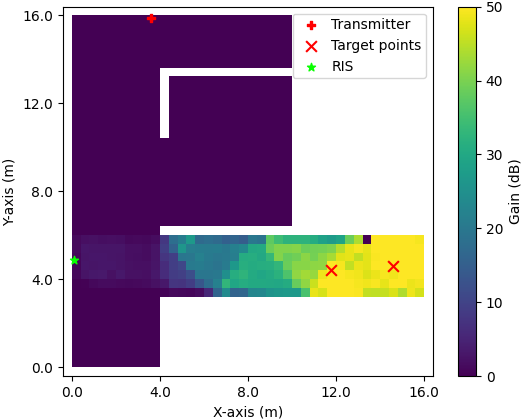
\includegraphics[width=0.49\linewidth]{Sim_Results/RIS_cov_gain_1x2_Gradient_-110dB.png}
	\hfill
	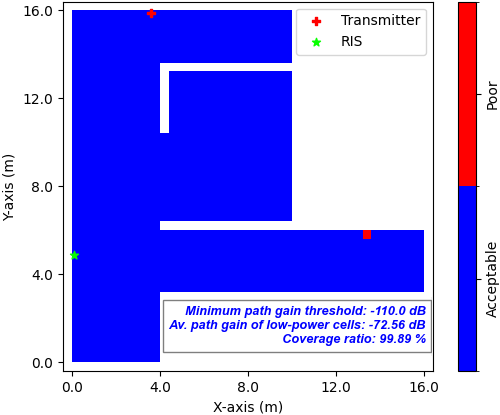
\includegraphics[width=0.48\linewidth]{Sim_Results/New_Binary_Cov_Map_1x2_Gradient_-110dB.png}
	
	b) RIS coverage gain \ \ \ \ \ \ \ \ \ \ \ c) New binary poor \\ \ \ \ \ \ \ \ \ \ \ \ \ \ \ \ \ \ \ \ \ \ \ \ \ \ \ \ \ \ \ \ \ \ \ \ \ \ \ \ coverage map
	\caption{Combined coverage map of the transmitter and the RIS with the RIS size of $1 \times 2$ m$^2$ by using the gradient-based approach for $-110$ dB minimum power threshold}
	\label{comb_cov_gradient_-110dB}
\end{figure}

\begin{figure}
	\centering
	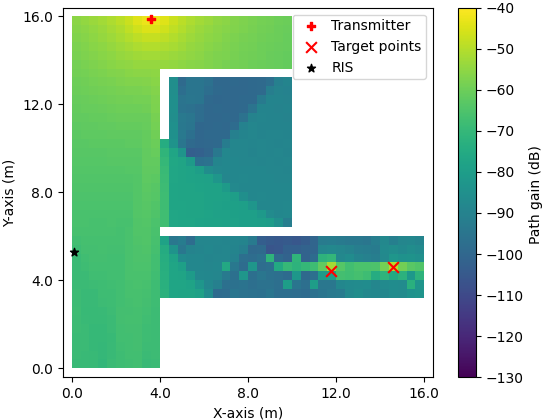
\includegraphics[width=0.7\linewidth]{Sim_Results/Comb_cov_1x2_Distance_-110dB.png}
	
	a) Combined coverage map \\[5pt]
	
	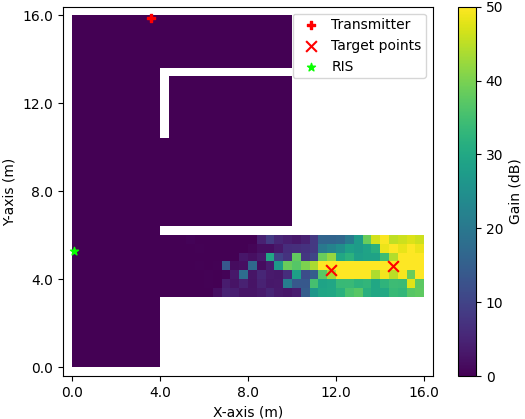
\includegraphics[width=0.49\linewidth]{Sim_Results/RIS_cov_gain_1x2_Distance_-110dB.png}
	\hfill
	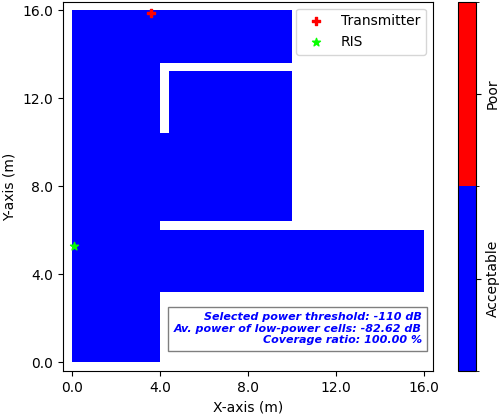
\includegraphics[width=0.48\linewidth]{Sim_Results/New_Binary_Cov_Map_1x2_Distance_-110dB.png}
	
	b) RIS coverage gain \ \ \ \ \ \ \ \ \ \ \ c) New binary poor \\ \ \ \ \ \ \ \ \ \ \ \ \ \ \ \ \ \ \ \ \ \ \ \ \ \ \ \ \ \ \ \ \ \ \ \ \ \ \ \ coverage map
	\caption{Combined coverage map of the transmitter and the RIS with the RIS size of $1 \times 2$ m$^2$ by using the distance-based approach for $-110$ dB minimum power threshold}
	\label{comb_cov_distance_-110dB}
\end{figure}

\section{CONCLUSION}

\begin{thebibliography}{00}
	\bibitem{sionna} J. Hoydis, S. Cammerer, Fayçal {A. A.}, A. Vem, N. Binder, G. Marcus, and A. Keller, “Sionna: An Open-Source Library for Next-Generation Physical Layer Research", \textit{arXiv}, March 2022, https://arxiv.org/abs/2203.11854.
	\bibitem{phase_grad_paper} E. M. Vitucci, M. Albani, S. Kodra, M. Barbiroli and V. Degli-Esposti, “An Efficient Ray-Based Modeling Approach for Scattering From Reconfigurable Intelligent Surfaces," \textit{IEEE Trans. on Antennas and Prop.}, vol. 72, no. 3, pp. 2673-2685, March 2024.
	\bibitem{Tang} W. Tang \textit{et al.}, “Wireless Communications With Reconfigurable Intelligent Surface: Path Loss Modeling and Experimental Measurement," \textit{IEEE Trans. on Wireless Commun.}, vol. 20, no. 1, pp. 421-439, Jan. 2021.
	\bibitem{emre_claude_eucap_paper} E. Kilcioglu and C. Oestges, “Ray-Tracing Based Algorithms for Indoor RIS Optimization and Coverage Enhancement," \textit{to appear in 2025 19th European Conference on Antennas and Propagation (EuCAP)}, 2025, pp. 1-5.
	\bibitem{ITU} ITU-R, “Effects of building materials and structures on radiowave propagation above about 100 MHz“, \textit{Recommendation ITU-R P.2040-2}. 
\end{thebibliography}


\begin{IEEEbiography}[{
\includegraphics[width=1in,height=1.25in,clip,keepaspectratio]{Emre_Picture.jpg}}]{EMRE KILCIOGLU } received his B.Sc. and M.Sc. degrees in Electrical and Electronics Engineering from Middle East Technical University, Ankara, Turkey, in 2016 and 2019, respectively. He completed his Ph.D. in 2024 at the Institute of Information and Communication Technologies, Electronics and Applied Mathematics (ICTEAM), Université catholique de Louvain (UCLouvain), Louvain-la-Neuve, Belgium, where he is currently a postdoctoral researcher. From July 2016 to January 2020, he worked as a system design engineer at Aselsan Inc., Ankara, Turkey. His research interests include massive MIMO, cooperative communication, deep learning applications in wireless communications, and ray-tracing-based optimization of reconfigurable intelligent surfaces (RISs).
\end{IEEEbiography}

\begin{IEEEbiography}[{
\includegraphics[width=1in,height=1.25in,clip,keepaspectratio]{Emre_Picture.jpg}}]{CLAUDE OESTGES } ...
\end{IEEEbiography}

\end{document}
